\subsection{Measurement}
\begin{frame}
	\frametitle\insertsection
	\framesubtitle\insertsubsection
	\vspace{-2em}
	\begin{block}{Definition}
		The term \textbf{measurement} contains all observed quantities included in a (possibly processed) report output from a sensor.
	\end{block}
\end{frame}
\begin{frame}
\frametitle\insertsection
	\framesubtitle\insertsubsection
	\begin{itemize}
		\item {Generic model of measurement}
		\begin{align*}
			y_{k} = h(x_{k}) + e_{k}
		\end{align*}
		\item {Example models}
		\begin{itemize}
			\item {Simple cartesian}
			\begin{align*}
				y_{k} =[x_{k} \ y_{k} ]^{T} + e_{k}
			\end{align*}
			\item {Range}
			\begin{align*}
				y_{k} =\sqrt{(x_k)^{2} + (y_k)^{2}} + e_k
			\end{align*}
			\item {Bearing only}
			\begin{align*}
				y_{k} = \arctan2(y_k,x_k)+ e_k
			\end{align*}
		\end{itemize}
	\end{itemize}
\end{frame}
\subsection{Tracks}
\begin{frame}
	\frametitle\insertsection
	\framesubtitle\insertsubsection
	\vspace{-2em}
	\begin{block}{Definition}
		A \textbf{track} is a sequence of measurements that has been decided or hypothesized by the tracker to come from a single source.
	\end{block}
	\begin{itemize}
		\item {Usually, instead of the list of actual measurements, sufficient statistics is held e.g., mean and covariance in the case of a KF, particles in the case of a PF.}
		\item {Generally each arriving measurement must start a track. Hence tracks must be classified and must not be treated equally.}
	\end{itemize}
	\end{frame}
\begin{frame}
	\frametitle\insertsection
	\framesubtitle\insertsubsection
	\vspace{-2em}
	\textbf{Track types:} According to their different life stages, tracks can be classified into 3 cases:
	\vspace{1em}
	\begin{itemize}
		\item {\textbf{Tentative} (initiator): A track that is in the track initiation process.
		This type cannot be sure that there is sufficient evidence that it is actually a target or not.}
		\item {\textbf{Confirmed:} A track that was decided to belong to a valid target in the surveillance area. This is one end of initiation process.}
		\item \textbf{Deleted:} At the other end of the initiation process, this is a track that is decided to come from all random false alarms or a target which can no longer be detected. All of its info should be deleted.
	\end{itemize}
\end{frame}
\begin{frame}
	\frametitle\insertsection
	\framesubtitle\insertsubsection
	\begin{itemize}
		\item {General state space model:}
		\begin{align*}
			x_{k}= f(x_{k-1})+w_{k}
		\end{align*}
		\item {Example models}
		\begin{itemize}
			\item {Constant Velocity}
			\begin{align*}
				x_{k}\triangleq
				\begin{bmatrix}
					x_k\\v^{x}_k
				\end{bmatrix} =
				\begin{bmatrix}
					1&T\\0&1
				\end{bmatrix}  
				\begin{bmatrix}
					x_{k-1}\\v^{x}_{k-1}
				\end{bmatrix} + 
				\begin{bmatrix}
					{T^{2}}/2\\T
				\end{bmatrix} a_k
			\end{align*}
			where $a_{k} \sim N(0, \sigma^{2}_{a})$ is a white noise.
		\end{itemize}
	\end{itemize}
\end{frame}
\begin{frame}
	\frametitle\insertsection
	\framesubtitle\insertsubsection
	\vspace{-2em}
	\begin{itemize}
		\item {Constant Velocity}
		\begin{align*}
			x_{k}\triangleq
			\begin{bmatrix}
				x_k\\v^{x}_k\\a^{x}_k
			\end{bmatrix} = 
			\begin{bmatrix}
				1&T&{T^2}/2 \\ 0&1&T \\ 0&0&1
			\end{bmatrix}
			\begin{bmatrix}
				x_{k-1}\\v^{x}_{k-1}\\a^{x}_{k-1}
			\end{bmatrix} + 
			\begin{bmatrix}
				{T^{2}}/{2} \\ T \\ 1
			\end{bmatrix}  \eta_{k}
		\end{align*}
		where $\eta _{k} \sim N(0, \sigma ^{2}_{ \eta })$ is a white noise.
	\end{itemize}
\end{frame}
\begin{frame}
	\frametitle\insertsection
	\framesubtitle\insertsubsection
	\vspace{-1em}
	\begin{itemize}
		\item {Coordinate Turn}
		\begin{align*}
			x_{k} &\triangleq
			\begin{bmatrix}
				x_k & y_k & v^{x}_k & v^{y}_k & \omega_k
			\end{bmatrix}^T \\
			&=
			\begin{bmatrix}
				1 & 0 &\cfrac{\sin(\omega_{k-1}T)}{\omega_{k-1}} & -\cfrac{1-\cos(\omega_{k-1}T) }{\omega_{k-1})} & 0 \\
				0 & 1 & \cfrac{1- \cos(\omega _{k-1}T) }{\omega_{k-1}} & \cfrac{\sin(\omega_{k-1}T) }{\omega_{k-1}} & 0 \\
				0 & 0 & \cos(\omega_{k-1}T) & -\sin(\omega_{k-1}T) & 0 \\
				0 & 0 & \sin(\omega_{k-1}T) & \cos(\omega_{k-1}T) & 0 \\
				0 & 0 & 0 & 0 & 1
			\end{bmatrix} x_{k-1}\\
			&\ \ +
			\begin{bmatrix}
				{T^{2}}/2 & 0 & 0 \\
				0 & {T^{2}}/2 & 0 \\
				T & 0 & 0 \\
				0 & T & 0 \\
				0 & 0 & 1
			\end{bmatrix} \eta _{k}
		\end{align*}
	\end{itemize}
\end{frame}
\subsection{Filtering}
\begin{frame}
	\frametitle\insertsection
	\framesubtitle\insertsubsection
	\vspace{-1em}
	When measurements corresponding to a target are obtained, the
	calculation of the sufficient statistics is done via state estimators (filters).
	\begin{itemize}
		\item {Early tracking systems: very low computational capacity => Steady state Kalman filters: $\alpha-\beta$ and $\alpha-\beta-\gamma$ filters. Kept an integer quality indicator instead of covariance.}
		\item {\textbf{Kalman filters} (KFs) and \textbf{Extended KFs} (EKF) are the most common approaches.}
		\item {\textbf{Unscented KF} (UKF) and other sigma-point approaches got much criticism (and undermining) from conservative" people in the field when they were first introduced. \textbf{Particle filters} (PFs) were despised.}
		\item {With the ever increasing computational resources, they are now commonly accepted as valid methods for target tracking.}
	\end{itemize}
\end{frame}
\subsection{Tracking Function}
\begin{frame}
	\frametitle\insertsection
	\framesubtitle\insertsubsection
	\vspace{-1em}
	\begin{itemize}
		\item {Correlation}
		\item {Association}
		\item {State Estimation}
		\item {Track Initiation \& Management}
	\end{itemize}
\end{frame}
\begin{frame}
	\frametitle\insertsection
	\framesubtitle\insertsubsection
	\vspace{-2em}
	\begin{figure}
		\caption{\textbf{Functional Diagram -- Tracking System}}
		\scalebox{1}{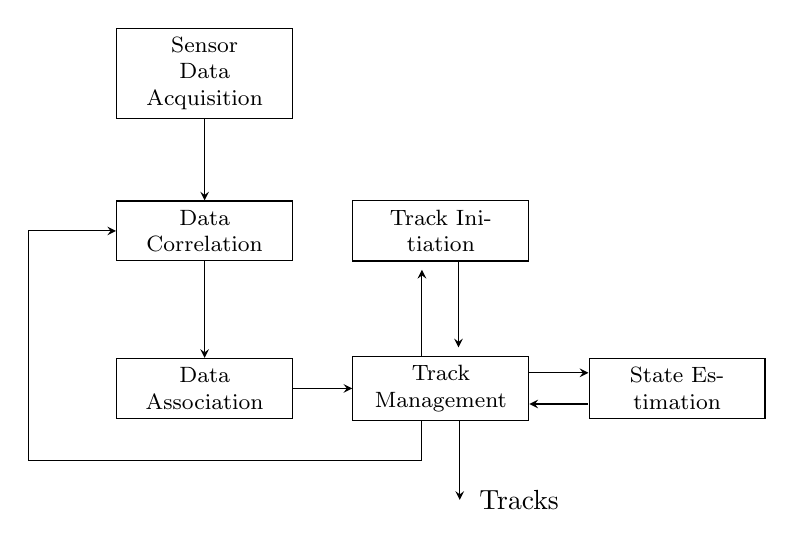
\begin{tikzpicture}[xscale=1,yscale=1,
	square/.style={rectangle, draw=black, text width=20mm, align=center, font=\footnotesize},
	label/.style={text width=5mm, align=center},
	node distance= 2cm, >=stealth]
	
	%Nodes
	\node[square]	(sda)	at (0,0) {Sensor\\Data\\Acquisition};
	\node[square]	(dc)	[below of=sda] {Data\\Correlation};
	\node[square]	(da)	[below of=dc] {Data\\Association};
	\node[square, xshift=1cm]	(ti)	[right of=dc] {Track Initiation};
	\node[square]	(tm)	[below of=ti] {Track\\Management};
	\node[square, xshift=1cm]	(se)	[right of=tm] {State Estimation};
	
	%Lines
	\draw[black, ->] (sda) -- (dc);
	\draw[black, ->] (dc) -- (da);
	\draw[black, ->] (da) -- (tm);
	\draw[black, ->] (ti.300) -- ++(0,-1.09);
	\draw[black, ->] (tm.120) -- ++(0,1.09);
	\draw[black, ->] (tm.10) -- ++(0.75,0);
	\draw[black, <-] (tm.350) -- ++(0.75,0);
	\draw[black, ->] (tm.240) -- ++(0,-0.5) -- ++(-5,0) |- (dc.west);
	\draw[black, ->] (tm.300) -- ++(0,-1) node[label, xshift=5mm] {Tracks};
\end{tikzpicture}}
	\end{figure}
\end{frame}
\begin{frame}
	\frametitle\insertsection
	\framesubtitle\insertsubsection
	\vspace{-2em}
	\begin{figure}
		\caption {\textbf{Tracking Process}}
		\scalebox{1}{\begin{tikzpicture}[xscale=1,yscale=1,
	round/.style={circle, inner sep=0pt, fill=red!50, opacity=0.75, align=center},
	point/.style={circle, inner sep=0pt, minimum size=2mm, align=center},
	oval/.style={ellipse, fill=green!50, opacity=0.75},
	label/.style={text width=15mm, align=center, font=\scriptsize},
	node distance= 3cm and 1cm, >=stealth]
		
	%Nodes
	\node[round, minimum size=3cm]	(acq)	at	(0,0)	{};
	\node[oval, minimum height=1.5cm, minimum width=3cm, rotate=45]	(window1)	at	(2,-2)	{};
	\node[oval, minimum height=1cm, minimum width=3cm, rotate=60]	(window2)	at	(4,-3)	{};
	\node[oval, minimum height=0.75cm, minimum width=3cm, rotate=75]	(window3)	at	(6,-3.5)	{};
	
	\node[point, minimum size=1.5mm, fill=blue!75]	(m1)	at	(0,0)	{};
	\node[point, minimum size=1.5mm, fill=blue!75]	(m2)	at	(1,-1)	{};
	\node[point, minimum size=1.5mm, fill=blue!75]	(m3)	at	(2.8,-1.75)	{};
	\node[point, minimum size=1.5mm, fill=blue!75]	(m4)	at	(4.75,-2.25)	{};
	\node[point, minimum size=1.5mm, fill=blue!75]	(m5)	at	(6.25,-3.6)	{};
	\node[point, minimum size=1.5mm, fill=red]	(e1)	at	(2.4, -1.875)	{};
	\node[point, minimum size=1.5mm, fill=red]	(e2)	at	(4.25, -2.75)	{};
	\node[point, minimum size=1.5mm, fill=red]	(e3)	at	(6.125, -3.55)	{};
	\node[point, minimum size=1.5mm, fill=gray]	(p1)	at	(2,-2)	{};
	\node[point, minimum size=1.5mm, fill=gray]	(p2)	at	(4,-3)	{};
	\node[point, minimum size=1.5mm, fill=gray]	(p3)	at	(6,-3.5)	{};
	
	%Labels
	\node[label]	(l1)	at	(2,1)		{Acquisition window};
	\node[label]	(l2)	at	(1.5,-3.5)	{Correlation window};
	\node[label, text width=18mm]	(l3)	at	(-1,-3)		{Predicted measurement};
	\node[label, text width=20mm]	(l4)	at	(3,0)		{State estimate};
	\node[label, text width=18mm]	(l5)	at	(-2,-1)		{New\\measurement};
	
	%Lines
	\draw[black, very thick, ->] (-0.5,0) -- (8,-4.25);
	\draw[black, densely dotted, -] (p1) -- (m3);
	\draw[blue!50, thick, -] (m1) -- (m2) -- (p1);
	\draw[blue!50, thick, -] (e1) -- (p2);
	\draw[blue!50, thick, -] (e2) -- (p3);
	\draw[black, densely dotted, -] (p2) -- (m4);
	\draw[blue!50, thick, ->] (e3) -- (7,-4);
	
	\draw[black, ->] (l3.north) -- (p1);
	\draw[black, ->] (l4) -- (e1);
	\draw[black, ->] (l5.north) -- (m1);
\end{tikzpicture}}
	\end{figure}
\end{frame}
